%prezentacja do pracy inżynierskiej (c) Kamil Strzempowicz
\documentclass{prezentacja}
\usepackage{mathtools}
\usepackage{color, colortbl}
\usepackage{graphicx}
%\usepackage{transparent}
\usepackage{wrapfig}
\usepackage{listings}

%\mathtoolsset{showonlyrefs}

\usetheme{lined} %motyw
\usecolortheme{dove}
%\useoutertheme[subsection=false]{miniframes}
\usepackage{etoolbox}
\makeatletter
\patchcmd{\slideentry}{\advance\beamer@xpos by1\relax}{}{}{}
\def\beamer@subsectionentry#1#2#3#4#5{\advance\beamer@xpos by1\relax}%
\makeatother

%%%%%%%%%%%%%%%%%%%%%%%
%%% Podstawowe info %%%
%%%%%%%%%%%%%%%%%%%%%%%

\title{Strategia Just in Time w systemach produkcyjnych\\ - analiza struktury gniazdowej dla heurystyk FIFO i LIFO}
\promotor{dr inż. Waldemar Grzechca}
\autor{Kamil Strzempowicz}
\author{Kamil Strzempowicz}
\subject{Subject}

\rodzPracy{Prezentacja projektu inżynierskiego}
\kierunek{Automatyka i Robotyka}
\institute{Wydział Automatyki, Elektroniki i Informatyki}

\setlength\intextsep{0pt}
\setlength{\wrapoverhang}{\marginparwidth}
\addtolength{\wrapoverhang}{\marginparsep}
\definecolor{darkGreen}{HTML}{006600}
\definecolor{lightGreen}{HTML}{66FF66}
\definecolor{lightRed}{HTML}{FF3300}
\definecolor{lightYellow}{HTML}{FFFF33}
\begin{document}
\lstset{
    language=C++,
    basicstyle=\scriptsize,
    tabsize=4,
    frame=lines,
    numbers=left,
    numberstyle=\tiny,
    numbersep=5pt,
    breaklines=true,
    showstringspaces=false,
    keywordstyle=\bfseries,
    commentstyle=\color{darkGreen}
}  

%%%%%%%%%%%%%%%%%%%%%%%%%%%%%%%%%
%%% początek właściwej treści %%%
%%%%%%%%%%%%%%%%%%%%%%%%%%%%%%%%%

\begin{frame}
    \StronaTyt
\end{frame}
\begin{frame}
    \frametitle{Spis tresci}
    \tableofcontents
\end{frame}
\section{Wstęp teoretyczny}
\subsection{Systemy gniazdowe}
\begin{frame}
    
    \begin{wrapfigure}{R}{.4\linewidth}
        \vspace{-110pt}
        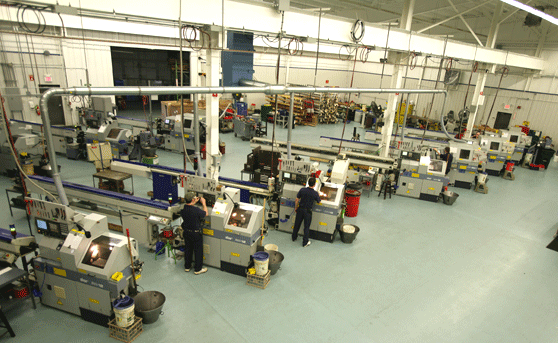
\includegraphics[width=\linewidth, keepaspectratio=true]{./obrazki/job-shop}
        \caption{\scriptsize Przykład systemu gniazdowego\cite{swiss}}
    \end{wrapfigure}
    
    \frametitle{Systemy gniazdowe}
    \vspace{60pt}
    Najczęściej wykorzystywane do pojedynczych zamówień, bądź krótkich serii. Takie systemy zwykle zmieniają swoje zastosowanie po zakończeniu każdego zlecenia. Zlecenie składa się ze skończonej liczby zadań, a~każde z~nich wymaga przeprowadzenia zestawu operacji na maszynach w~ustalonym porządku, innym dla każdego zadania.
    
   

\end{frame}
\subsection{Strategia Just in Time}
\begin{frame}
    \frametitle{Strategia Just in Time}
    Zadanie powinno być ukończone możliwie blisko swojego terminu zakończenia (due date) jak to tylko możliwe. Zbyt wczesne zakończenie zadania pociąga za sobą koszty utrzymania, takie jak magazynowania czy ubezpieczenia. Z~drugiej jednak strony spóźnione zlecenie często skutkuje karami umownymi czy nadszarpnięciem reputacji przedsiębiorstwa \cite{genetyczne}.

    Na potrzeby tej pracy wybrano następujące funkcje matematycznie opisujące dostosowanie uszeregowania do strategii JIT:
\small{
    \begin{equation}
        \sqrt{\sum e_j^2 + \sum l_j^2}
        \label{eq:w1}
    \end{equation}
    \begin{equation}
        \alpha*\sum e_j + \beta*\sum l_j
        \label{eq:w2}
    \end{equation}
}
\footnotesize{
    \begin{tabular}{r l}    
    \(e_j\) & przedwczesność j-tego zadania, \\
    \(l_j\) & spóźnienie j-tego zadania, \\
    \(\alpha, \beta\) & wagi przedwczesności i~spóźnienia.
    \end{tabular}
}
\end{frame}
\section{Program kSzereg}
\subsection{Opis}
\begin{frame}   
    \begin{wrapfigure}{r}{.4\linewidth}
        \vspace{-60pt}
        
\includegraphics[width=\linewidth, keepaspectratio=true]{./obrazki/QtLogo}
    \end{wrapfigure}
    
    \frametitle{Program kSzereg}
    Program kSzereg został napisany w~C++ na potrzeby tej pracy dyplomowej. Umożliwia on przeprowadzenie szeregowania zadań w~systemie wytwarzania gniazdowego na podstawie heurystyki \emph{First In First Out} (FIFO) bądź \emph{Last In First Out} (LIFO). 
    
    Wprowadzanie danych odbywa się za pośrednictwem graficznego interface'u opartego o~framework Qt\cite{qt}.
    
    Kod żródłowy programu kSzereg jest publicznie dostępny na zasadach licencji GNU GPL\cite{gpl} w sewisie bitbucklet\cite{bit}. 
    
\end{frame}
\begin{frame}[fragile]
    \begin{columns}
        \begin{column}{.55\textwidth}
            \footnotesize
            Aktualnie program kSzereg umożliwia szeregowanie w oparciu o następujące heurystyki:
            \begin{itemize}
                \normalsize
                \item\emph{FIFO} - Pierwsze jest przetwarzane zadanie, które wpłynęło najwcześniej\cite{jobSlack}.
                \item\emph{LIFO} - Pierwsze jest przetwarzane zadanie, które wpłynęło najpóźniej\cite{jobSlack}.
            \end{itemize}
            Został on jednak tak zaprojektowany, aby umożliwić łatwą rozbudowę o kolejne heurystyki. 
        \end{column}
        \begin{column}{.45\textwidth}
            \frametitle{Heurystyki}
            \begin{lstlisting}
switch(method)
{
case 0://fifo
    start(kolejka.first());
    kolejka.removeFirst();
    break;
case 1://lifo
    start(kolejka.last());
    kolejka.removeLast();
    break;
}
            \end{lstlisting}
        \end{column}
    \end{columns}
\end{frame}
\subsection{Zrzuty ekranu}
\def\ofset{1.4cm}
\hspace{-\ofset}
\begin{frame}
    \frametitle{\hspace{\ofset}Główne okno}
    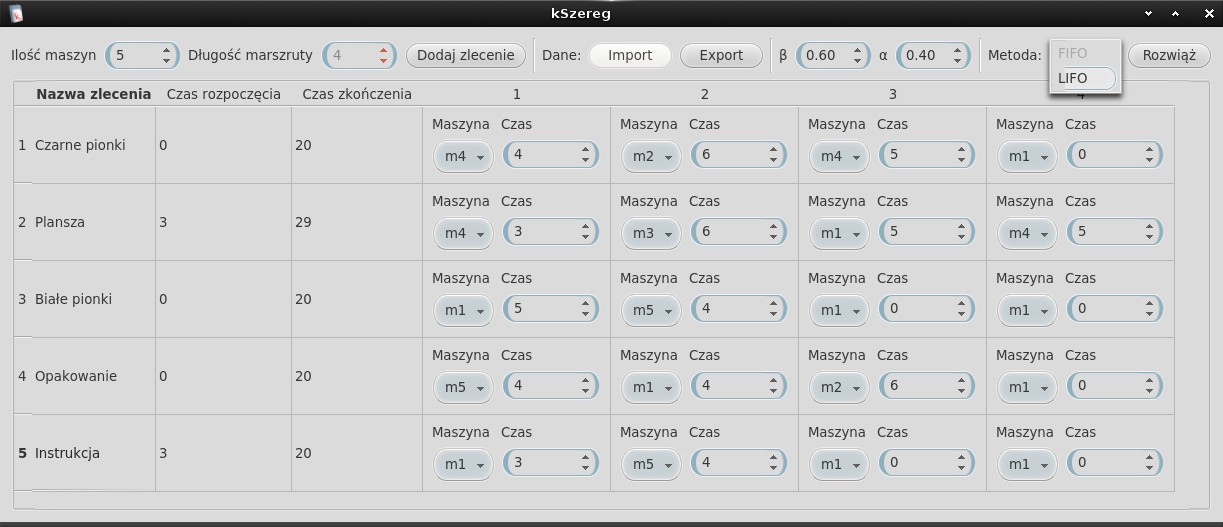
\includegraphics[width=\paperwidth-.45cm, keepaspectratio=true]{./obrazki/s1}
\end{frame}
\begin{frame}
    \frametitle{Okno rozwiązania}
    \begin{figure}[htb]
        \centering
        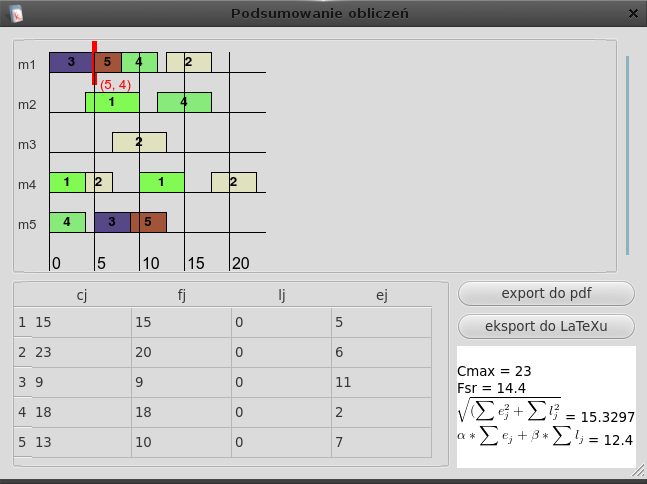
\includegraphics[height=.8\textheight, keepaspectratio=true]{./obrazki/s2}
    \end{figure}    
\end{frame}
\begin{frame}
    \frametitle{Linia poleceń}
    \begin{figure}[htb]
        \centering
        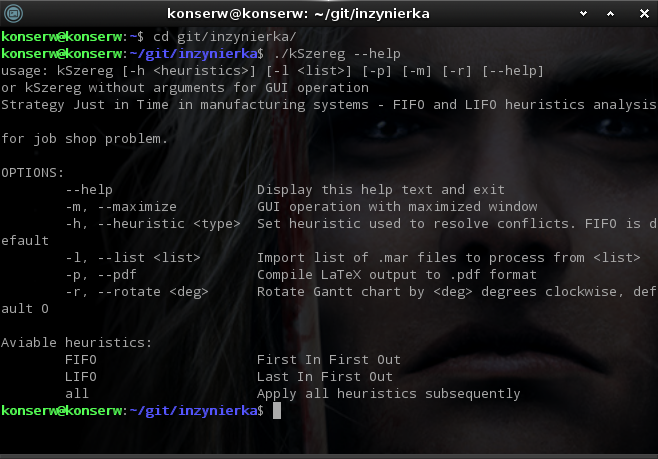
\includegraphics[height=.8\textheight, keepaspectratio=true]{./obrazki/s3}
    \end{figure}  
\end{frame}

\section{Zastosowanie programu kSzereg}
\subsection     {Badanie zlecenia}
\label{sec:z1}
\begin{frame}
    \frametitle{Badanie zlecenia}
    \begin{table}[htb]
		\centering
		\caption{\large Struktura zlecenia}
		\begin{tabular}{ | r | c | c | l | }
		\hline
		j	& \(r_j\)	& \(d_j\)	& Marszruta technologiczna	\\ \hline
		1	& 10	& 55	& m4 (8) - m7 (6) - m9 (7) - m8 (3) - m1 (6)	\\ \hline
		2	& 0	& 45	& m5 (4) - m4 (8) - m2 (6) - m8 (6) - m9 (7)	\\ \hline
		3	& 5	& 50	& m8 (7) - m2 (7) - m7 (7) - m3 (5) - m1 (4)	\\ \hline
		4	& 0	& 40	& m5 (10) - m9 (5) - m4 (6) - m1 (6) - m6 (2)	\\ \hline
		5	& 5	& 45	& m1 (4) - m5 (10) - m9 (7) - m4 (7) - m2 (5)	\\ \hline
		6	& 0	& 40	& m8 (6) - m6 (7) - m9 (6) - m2 (6) - m6 (12)	\\ \hline
		7	& 5	& 45	& m4 (8) - m2 (6) - m3 (7) - m7 (8) - m6 (3)	\\ \hline
		\end{tabular}
	\end{table}
\end{frame}
\begin{frame}
    \frametitle{Wyznaczniki jakości uszeregowań}
    \begin{table}[htb]
        \caption{Heurystyka FIFO}
        \scriptsize
        \centering
        \begin{tabular}{ l l l }
            \(C_{max} = 55 \)	& \( T_{max} = 10 \)	& \( \sqrt{\sum e_j^2 + \sum l_j^2} = 19.799\)	\\
            \( \bar{F} = 42.4286 \)	& \( \bar{T} = 3.28571 \)	& \( \alpha*\sum e_j + \beta*\sum l_j \Big|_{\substack{\alpha = 0.2\\ \beta = 0.8}} = 22.6 \)	\\ 
        \end{tabular}
    \end{table}
	
    \begin{table}[htb]
        \caption{Heurystyka LIFO}
        \scriptsize
		\centering
		\begin{tabular}{ l l l }
		\(C_{max} = 54 \)	& \( T_{max} = 9 \)	& \( \sqrt{\sum e_j^2 + \sum l_j^2} = 17.5499\)	\\
		\( \bar{F} = 44.4286 \)	& \( \bar{T} = 3.85714 \)	& \( \alpha*\sum e_j + \beta*\sum l_j \Big|_{\substack{\alpha = 0.2\\ \beta = 0.8}} = 23.8 \)	\\ 
		\end{tabular}
	\end{table}
\end{frame}

\subsection     {Zmodyfikowane zlecenie ze zmienioną marszrutą}
\label{sec:z2}
\begin{frame}
    \frametitle{Zmodyfikowane zlecenie ze zmienioną marszrutą}
    \begin{table}[htb]
		\centering
		\caption{Struktura zlecenia}
		\scriptsize
		\begin{tabular}{ | r | c | c | l | }
		\hline
		j	& \(r_j\)	& \(d_j\)	& Marszruta technologiczna	\\ \hline
		1	& 10	& 55	& m4 (8) - m7 (6) - m9 (7) - m8 (3) - m1 (6)	\\ \hline
		2	& 0	& 45	& m5 (4) - m4 (8) - m2 (6) - m8 (6) - m9 (7)	\\ \hline
		3	& 5	& 50	& m8 (7) - m2 (7) - m7 (7) - m3 (5) - m1 (4)	\\ \hline
\rowcolor{lightYellow}
		4	& 0	& 40	& m5 (10) - m9 (5) - m4 (6) - m1 (6) - m5 (4)	\\ \hline
		5	& 5	& 45	& m1 (4) - m5 (10) - m9 (7) - m4 (7) - m2 (5)	\\ \hline
		6	& 0	& 40	& m8 (6) - m6 (7) - m9 (6) - m2 (6) - m6 (12)	\\ \hline
\rowcolor{lightYellow}
		7	& 0	& 45	& m4 (8) - m2 (6) - m3 (7) - m7 (8) - m6 (3)	\\ \hline
		\end{tabular}
	\end{table}    
    \begin{table}[htb]
        \caption{Wyznaczniki jakości uszeregowania LIFO}
        \scriptsize
        \centering
        \begin{tabular}{ l l l }
		\(C_{max} = 51 \)	& \( T_{max} = 6 \)	& \( \sqrt{\sum e_j^2 + \sum l_j^2} = 14.4222\)	\\
		\( \bar{F} = 40.2857 \)	& \( \bar{T} = 0.857143 \)	& \( \alpha*\sum e_j + \beta*\sum l_j \Big|_{\substack{\alpha = 0.2\\ \beta = 0.8}} = 9.6 \)	\\ 
        \end{tabular}
    \end{table}
\end{frame}

\subsection     {Zmodyfikowane zlecenie bez zmian w marszrucie}
\label{sec:z3}
\begin{frame}
    \frametitle{Zmodyfikowane zlecenie bez zmian w marszrucie}
    \begin{table}[htb]
		\centering
		\caption{\large Struktura zlecenia}
		\scriptsize
		\begin{tabular}{ | r | c | c | l | }
		\hline
		j	& \(r_j\)	& \(d_j\)	& Marszruta technologiczna	\\ \hline
		1	& 10	& 55	& m4 (8) - m7 (6) - m9 (7) - m8 (3) - m1 (6)	\\ \hline
		2	& 0	& 45	& m5 (4) - m4 (8) - m2 (6) - m8 (6) - m9 (7)	\\ \hline
		3	& 5	& 50	& m8 (7) - m2 (7) - m7 (7) - m3 (5) - m1 (4)	\\ \hline
		4	& 0	& 40	& m5 (10) - m9 (5) - m4 (6) - m1 (6) - m6 (2)	\\ \hline
		5	& 5	& 45	& m1 (4) - m5 (10) - m9 (7) - m4 (7) - m2 (5)	\\ \hline
		6	& 0	& 40	& m8 (6) - m6 (7) - m9 (6) - m2 (6) - m6 (12)	\\ \hline
		\rowcolor{lightYellow}
		7	& 0	& 45	& m4 (8) - m2 (6) - m3 (7) - m7 (8) - m6 (3)	\\ \hline
		\end{tabular}
	\end{table}    
    \begin{table}[htb]
        \caption{\large Wyznaczniki jakości uszeregowania LIFO}
        \scriptsize
        \centering
        \begin{tabular}{ l l l }
		\(C_{max} = 62 \)	& \( T_{max} = 17 \)	& \( \sqrt{\sum e_j^2 + \sum l_j^2} = 23.2379\)	\\
		\( \bar{F} = 42.7143 \)	& \( \bar{T} = 4.85714 \)	& \( \alpha*\sum e_j + \beta*\sum l_j \Big|_{\substack{\alpha = 0.2\\ \beta = 0.8}} = 30.4 \)	\\ 
        \end{tabular}
    \end{table}
\end{frame}
\subsection{Zmodyfikowane zlecenie z naciskiem na $e_j$ }
\label{sec:z4}
\begin{frame}
    \frametitle{Zmodyfikowane zlecenie z naciskiem na $e_j$ }
    \begin{table}[htb]
		\centering
		\caption{\large Struktura zlecenia}
		\scriptsize
		\begin{tabular}{ | r | c | c | l | }
		\hline
		j	& \(r_j\)	& \(d_j\)	& Marszruta technologiczna	\\ \hline
		\rowcolor{lightYellow}
		1	& 14	& 55	& m4 (8) - m7 (6) - m9 (7) - m8 (3) - m1 (6)	\\ \hline
		\rowcolor{lightYellow}
		2	& 3	& 45	& m5 (4) - m4 (8) - m2 (6) - m8 (6) - m9 (7)	\\ \hline
		\rowcolor{lightYellow}
		3	& 12	& 50	& m8 (7) - m2 (7) - m7 (7) - m3 (5) - m1 (4)	\\ \hline
		4	& 0	& 40	& m5 (10) - m9 (5) - m4 (6) - m1 (6) - m6 (2)	\\ \hline
		5	& 5	& 45	& m1 (4) - m5 (10) - m9 (7) - m4 (7) - m2 (5)	\\ \hline
		6	& 0	& 40	& m8 (6) - m6 (7) - m9 (6) - m2 (6) - m6 (12)	\\ \hline
		7	& 5	& 45	& m4 (8) - m2 (6) - m3 (7) - m7 (8) - m6 (3)	\\ \hline
		\end{tabular}
	\end{table}    
    \begin{table}[htb]
        \caption{\large Wyznaczniki jakości uszeregowania FIFO}
        \scriptsize
        \centering
        \begin{tabular}{ l l l }
		\(C_{max} = 58 \)	& \( T_{max} = 7 \)	& \( \sqrt{\sum e_j^2 + \sum l_j^2} = 15.3948\)	\\
		\( \bar{F} = 43.2857 \)	& \( \bar{T} = 2.85714 \)	& \( \alpha*\sum e_j + \beta*\sum l_j \Big|_{\substack{\alpha = 0.2\\ \beta = 0.8}} = 19.4 \)	\\ 
        \end{tabular}
    \end{table}
\end{frame}


\section{Wnioski}
\begin{frame}
    \frametitle{Wnioski}
    Porównanie wyznaczników jakości uszeregowania
    \begin{table}[htb]
	    \centering
	    \scriptsize
	    \begin{tabular}{ r | c | c | c | c | c | c }
	    zlecenie       & \(C_{max}\)	& \(\bar{F}\)   & \(T_{max}\) & \(\bar{T}\) & funkcja \eqref{eq:w1} & funkcja \eqref{eq:w2} \\ \hline
	    \ref{sec:z1} FIFO & \cellcolor{lightRed} 55 & 42,4286 & \cellcolor{lightRed} 10 & 3,28571 & \cellcolor{lightRed} 19,7999 & 22,6 \\ \hline
	    \ref{sec:z1} LIFO & 54 & \cellcolor{lightRed}44,4286 & 9 & \cellcolor{lightRed} 3,85714 & 17,5499 & \cellcolor{lightRed} 23,8 \\ \hline
        \ref{sec:z2} LIFO & \cellcolor{lightGreen} 51 & \cellcolor{lightGreen} 40,2857 & \cellcolor{lightGreen} 6  & \cellcolor{lightGreen} 0,857143 & 14,4222 & \cellcolor{lightGreen} 9,6  \\ \hline
	    \ref{sec:z3} LIFO & \cellcolor{lightGreen} 51 & 41,7143       & 6           & 1,42857      & 13,7113      & 11,6 \\ \hline
	    \ref{sec:z4} FIFO & 54          & 42,8571       & 9           & 3,71429      & \cellcolor{lightGreen} 13,5277 & 22,2 \\ 
	    \end{tabular}
    \end{table}
\end{frame}
\section{Literatura}
\begin{thebibliography}{1}
\begin{frame}
    \frametitle{Literatura}
    \scriptsize
    
    \bibitem{swiss}
    \emph{Strona internetowa firmy Swissturn},
    Źródło: \url{http://www.swissturn.com} [dostęp:~21.01.2013]

    \bibitem{genetyczne}
    Rodolfo Pereira Araujo, André Gustavo dos Santos, José Elias Cláudio Arroyo,
    \emph{Genetic Algorithm and Local Search for Just-in-Time Job–Shop Scheduling},
    2009 IEEE Congress on Evolutionary Computation (CEC 2009)

    \bibitem{qt}
    \emph{Strona internetowa projektu Qt},
    Źródło: \url{http://qt.digia.com/} [dostęp:~21.01.2013]

    \bibitem{gpl}
    \emph{Strona internetowa projektu GNU},
    Źródło: \url{http://www.gnu.org/licenses/} [dostęp:~21.01.2013]

    \bibitem{bit}
    \emph{Repozytorium programu kSzereg},
    Żródło: \url{https://bitbucket.org/konserw/kszereg} [dostęp:~21.01.2013]

    \bibitem{jobSlack}
    M. G. C. Resende,  
    \emph{Shop Floor Scheduling of Semiconductor Wafer Manufacturing},
    PhD thesis Department of Industrial Engineering and Operations Research, University of California, Berkeley, 1987 
\end{frame}
\end{thebibliography}
\end{document}        
